\subsubsection{\stid{1.14} GASNet-EX}\label{subsubsect:gasnet-ex}
\paragraph{Overview} 

GASNet-EX~\cite{gasnet-site} is a portable high-performance communication layer
supporting multiple implementations of the Partitioned Global Address Space
(PGAS) model.
GASNet-EX clients include Pagoda's PGAS programming interface UPC++~\cite{upcxx-ipdps19,upcxx-site}
 and the Legion Programming
System~\cite{bauer2012legion,legion-site} (WBS~2.3.1.08).

GASNet-EX's low-overhead communication mechanisms are designed to maximize
injection rate and network utilization, tolerate latency through
overlap, streamline unpredictable communication events, minimize
synchronization,
leverage hardware support for communication involving accelerator memory,
and efficiently support small- to medium-sized
messages arising in ECP applications.  GASNet-EX enables the ECP
software stack to exploit the best-available communication mechanisms,
including novel features still under development by vendors.  The
GASNet-EX communications library and the PGAS models built upon it
offer a complementary, yet interoperable, approach to ``MPI + X'',
enabling developers to focus their effort on optimizing
performance-critical communication.

We are co-designing GASNet-EX with the UPC++ development team,
along with additional input from the Legion and
(non-ECP) Cray Chapel~\cite{chapel-chapter,chapel-site} projects.

\paragraph{Key Challenges}

Exascale systems will deliver exponential growth in on-chip parallelism and
reduced memory capacity per core, 
increasing the importance of strong
scaling and finer-grained communication events.  
Success at exascale demands minimizing software overheads,
especially avoiding long, branchy serial code paths; 
this motivates a requirement for efficient
fine-grained communication.
The pervasive use of accelerators introduces heterogeneous systems including
memory with properties that differ from host DRAM but can still benefit from
network offload support during communication.
These challenges are exacerbated by application trends; many of the ECP applications require
adaptive meshes, sparse matrices,
or dynamic load balancing.
All of these characteristics favor the use of
low-overhead communication mechanisms that
can maximize injection rate and network utilization, tolerate latency through
overlap, accommodate unpredictable communication events, minimize synchronization,
leverage hardware support for communication involving accelerator memory,
and efficiently support small- to medium-sized messages. The ECP software stack
needs to expose the best-available communication mechanisms, including novel
features being developed by the vendor community.

\paragraph{Solution Strategy}

The PGAS model is a powerful means of addressing these
challenges and is critical in building other ECP programming systems,
libraries, and applications.  We use the term PGAS for models that support
one-sided communication, 
including contiguous and non-contiguous remote memory access (RMA) operations such as put/get
and atomic updates. Some of these models also include support for remote function invocation.
GASNet-EX~\cite{gasnet-lcpc18} is a communications library that provides the foundation for implementing
PGAS models, and is the successor to the widely-deployed GASNet library.
We are building on over 20 years of experience with the GASNet~\cite{gasnet-site,gasnet-spec}
communication layer to provide production-quality implementations that include
improvements motivated by
technology trends and application experience.  

The goal of the GASNet-EX team is to provide a portable, high-performance PGAS
communication layer for exascale and pre-exascale systems, addressing the challenges
identified above.
GASNet-EX provides interfaces that efficiently match the RDMA capabilities of modern
inter-node network hardware and intra-node communication between distinct address spaces.
New interfaces for atomics and collectives have enabled offload to current
and future network hardware with corresponding capabilities.
New interfaces for non-host memory are designed to enable efficient transfers
to and from device memories, by leveraging such vendor technologies as
GPUDirect RDMA (GDR).
Together these design choices and their implementations supply the low-overhead communication
mechanisms required to address the requirements of exascale applications.

\begin{figure}[htb]
  \centering
  \subfloat[8-byte RMA Latencies\label{fig:rma-lat-bars}]{
     \includegraphics[width=0.432\textwidth]{projects/2.3.1-PMR/2.3.1.14-UPCxx-GASNet/latency_bars.pdf}
  }
  \subfloat[Summit Flood Bandwidth\label{fig:summit-bw}]{
     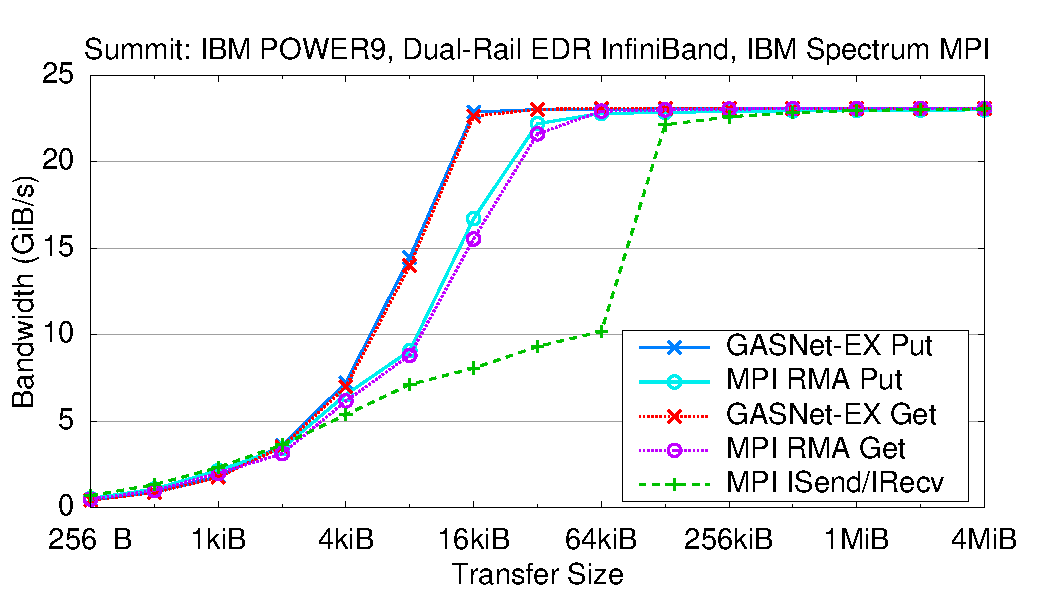
\includegraphics[width=0.504\textwidth]{projects/2.3.1-PMR/2.3.1.14-UPCxx-GASNet/Summit-slide-BW.pdf}
  }
  \caption{\label{fig:gasnet-ex-rma} Selected GASNet-EX vs. MPI RMA Performance Results}
\end{figure}

Figure~\ref{fig:gasnet-ex-rma} shows representative results from a
paper~\cite{gasnet-lcpc18} comparing
the RMA performance of GASNet-EX against MPI on multiple systems including
NERSC's Cori and OLCF's Summit.%
\footnote{The paper's results from Summitdev
have been replaced by more recent (June 2019) results from OLCF's newer Summit system.}
These results demonstrate the ability of a PGAS-centric runtime to
deliver performance as good as MPI, and often better.
%
The paper presents experimental methodology and system descriptions, which are
also available online~\cite{gasnet-site}, along with results for additional
systems.

Figure~\ref{fig:rma-lat-bars} shows the latency of 8-byte RMA Put and Get operations on
four systems, including two distinct network types and three distinct MPI
implementations.
%
GASNet-EX's latency is 6\% to 55\% better than MPI's on Put and 5\% to 45\%
better on Get.
%
Algorithms sensitive to small-transfer latency may become practical in PGAS
programming models due to these improvements relative to MPI.
%
Figure~\ref{fig:summit-bw} shows flood bandwidth of RMA Put and Get measured
on OLCF's Summit.
GASNet-EX's bandwidth is seen to rise to saturation at smaller
transfer sizes than IBM Spectrum MPI, with the most pronounced differences
appearing between 4KiB and 32KiB.
%
Comparison to the bandwidth of MPI message-passing (dashed green) illustrates the
benefits of one-sided communication, a major feature of PGAS models.


\paragraph{Recent Progress}

The most notable work on GASNet-EX in the past year has been in device memory support and tuning.

\subparagraph{Device (GPU) Memory Support}
Memory kinds is the GASNet-EX term for support of communication involving
memory other than host memory.  In the context of ECP, the primary focus is
accelerator devices such GPUs.  However, the design is extensible to other
accelerators, such as FPGAs, and to storage.
Since late 2020, GASNet-EX has leveraged the GDR
capabilities of modern NVIDIA GPUs and Mellanox network adapters (such as those
on Summit) to perform one-sided RMA involving GPU memory without
the overheads of staging through intermediate buffers in host memory.
The GASNet-EX APIs for memory kinds have been co-designed with the developers
of UPC++ and the Realm runtime layer of the Legion Programming System
(WBS~2.3.1.08), and both projects have leveraged this support since
their respective late 2020 releases.
Performance of GASNet-EX memory kinds, including via Legion and UPC++
benchmarks, is featured on an SC21 research poster~\cite{gasnet-poster-sc21},
and additional UPC++ performance results using memory kinds appear in
Figure~\ref{fig:paw21_interop_strong_scaling} in
Section~\ref{subsubsect:upcxx}.
The most recent work on memory kinds has extended the implementation in two directions:
adding support for the UCX network API and for GPUs using the AMD HIP API.
The net result is support for four combinations of network API and GPU vendor.

\subparagraph{Tuning}
We have devoted effort in the past year to improving the performance and memory
use of the GASNet-EX runtime.  Examples of this work include significant
improvements to InfiniBand support which (1) reduce memory consumption at large
job sizes and (2) improve scaling to large thread counts in multi-threaded
clients.  Other recent tuning efforts have reduced the overheads for put, get
and atomic updates in intra-node shared memory.

\paragraph{Preliminary Results on Early Access Systems}

Early access to OLCF's HPE Cray EX systems, Spock and Crusher, have helped our
team to pursue support in GASNet-EX for their respective networks (Slingshot-10
and Slingshot-11) and for efficient RMA transfers to and from AMD GPUs.

Experiences on OLCF's Spock system helped to enable the recent addition of
memory kinds support for the UCX network API and for GPUs using the AMD HIP API.
In particular, use of the ROCmRDMA technology allows network hardware to
perform RMA operations to and from memory on AMD GPUs without staging through
buffers in host memory.
%
Microbenchmarks collected on Spock of RMA put operations from local host memory
to remote GPU memory show bandwidth peaking to the same 11.4GiB/s as for
transfers in either direction between host memory at both ends.
Meanwhile, RMA get operations from remote GPU memory to local host memory reach
a peak bandwidth of 9.3GiB/s.  
%
Figure~\ref{fig:upcxx-spock} in Section~\ref{subsubsect:upcxx}
shows preliminary results for a UPC++ benchmark run on Spock, which illustrate
how leveraging the new ROCmRDMA support in GASNet-EX translates into significant
performance gains over the prior implementation approach.

Early experiences on OLCF's Crusher system are driving development of support
for the HPE Slingshot-11 network.  This work is anticipated to appear in the
Spring 2022 release of GASNet-EX.  Preliminary results have demonstrated the
ability of GASNet-EX to effectively utilize all four network interfaces in a
Crusher node, and to deliver peak RMA bandwidths competitive with those HPE
has reported for their MPI on comparable transfers.

\paragraph{Next Steps}

Next steps for each effort have already been identified.

\subparagraph{Device (GPU) Memory Support}
We will continue work in the area of GASNet-EX memory kinds, including the
hardening and tuning of the current implementation.
As access to relevant systems is secured, we plan to extend support to
additional accelerators and networks, with Intel GPUs and the HPE Slingshot
network being the most important examples for ECP.

\subparagraph{Client-Driven Tuning}
In collaboration with authors of client runtimes using GASNet-EX (most notably
UPC++ and Legion) and their users (such as ExaBiome), we will continue to
identify and address any significant scalability issues or performance
anomalies which are discovered.

%\clearpage
